\section{Reduction to the critical mean}\label{sec:reduction}

Fix an integer $k\ge2$. We follow the critical-mean reduction of Chi, Sun, and Wang~\cite[Section 2.1]{CSW2026}. We first identify the mean at which the two proposed extremal distributions give the same probability. We then show that a proof at this mean determines both the optimal value and the maximizing distributions at every other mean.

For $c\ge0$, define
\begin{align*}
 g_k(c)\coloneqq \left(1+\frac ck\right)^k-\left(1+\frac{c-1}{k}\right)^k.
\end{align*}
Its derivative is positive, $g_k(0)<1$, and $g_k(1)>1$. Thus there is a unique $c_k\in(0,1)$ such that $g_k(c_k)=1$. Define
\begin{align}\label{eq:critical-parameters}
 \beta_k\coloneqq\frac1{k+c_k}.
\end{align}
For $x\in(0,1/k)$, substituting $c=1/x-k$ gives
\begin{align*}
 1-(1-x)^k-(kx)^k=(kx)^k\bigl(g_k(c)-1\bigr).
\end{align*}
Consequently, $\beta_k$ is the unique crossing point of the two proposed bounds in $(0,1/k)$; the Bernoulli expression is larger for $x<\beta_k$, and the other expression is larger for $x>\beta_k$.

For example, when $k=3$, the crossing equation reduces to $26\beta_3^2+3\beta_3-3=0$, so $\beta_3=(\sqrt{321}-3)/52$. The two candidate probabilities are shown in \cref{fig:critical-mean}. The reduction below explains why proving the bound at their intersection is sufficient.
\begin{figure}[ht]
\centering
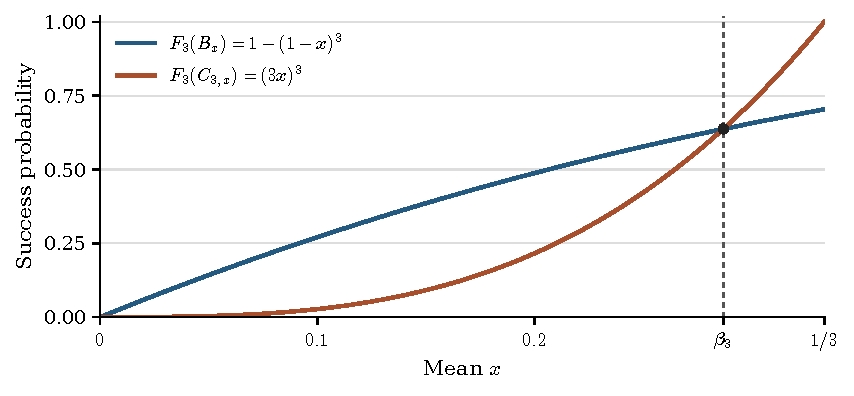
\includegraphics[width=0.76\textwidth]{figures/critical_mean.pdf}
\caption{The two candidate probabilities when $k=3$. Their unique intersection in $(0,1/3)$ occurs at $\beta_3\approx0.286855$. The larger curve gives the sharp bound.}
\label{fig:critical-mean}
\end{figure}

We will repeatedly use $c_k\le1/2$, with equality only when $k=2$. To see this, expand $g_k(1/2)$ about $1$:
\begin{align*}
 g_k(1/2)=2\sum_{\substack{h\in[k]\\ h\text{ odd}}}\binom kh(2k)^{-h}.
\end{align*}
The term with $h=1$ is $1$. The remaining terms vanish when $k=2$ and include a positive term when $k\ge3$. The assertion follows from the strict increase of $g_k$.

The following two mixing operations explain why the crossing point is the appropriate mean to study. For any nonnegative law $P$ and $0\le\vartheta,q\le1$, independence gives
\begin{align}
 1-F_k\bigl((1-\vartheta)P+\vartheta\delta_1\bigr)
   &=(1-\vartheta)^k\bigl(1-F_k(P)\bigr),\label{eq:mix-one}\\
 F_k\bigl(qP+(1-q)\delta_0\bigr)
   &=\sum_{j\in[k]}\binom kj q^j(1-q)^{k-j}F_j(P)
     \ge q^kF_k(P).\label{eq:mix-zero}
\end{align}
For the first identity, failure requires that none of the $k$ samples come from the added atom at $1$. For the second, condition on the number of samples drawn from $P$; a sample drawn from the added atom contributes zero.

Suppose for the moment that the proposed upper bound has been proved at mean $\beta_k$. If $m(P)=x<\beta_k$, set $\vartheta=(\beta_k-x)/(1-x)$. The mixed law in \cref{eq:mix-one} has mean $\beta_k$, and $1-\vartheta=(1-\beta_k)/(1-x)$. It follows that
\begin{align*}
 (1-\vartheta)^k\bigl(1-F_k(P)\bigr)\ge(1-\beta_k)^k,
 \qquad F_k(P)\le1-(1-x)^k.
\end{align*}
If $\beta_k<x<1/k$, set $q=\beta_k/x$. Applying the critical-mean bound to \cref{eq:mix-zero} gives $q^kF_k(P)\le(k\beta_k)^k$, and hence $F_k(P)\le(kx)^k$. A law with mean less than $x<1/k$ can first be mixed with $\delta_1$ to raise its mean to $x$. This does not decrease its success probability. The cases $x=0$ and $x\ge1/k$ will be treated together with equality in \cref{sec:equality}.

Before studying the critical mean, we establish existence and a useful description of every maximizing law. These conclusions are given in Chi, Sun, and Wang~\cite[Lemma 2.7 and Proposition 2.10]{CSW2026}. The proof below obtains the normalization by an elementary truncation and rescaling argument. The description supplies the atom at zero that is needed for the variations used later.

\begin{lemma}\label{lem:normalization}
Let $0<x<1/k$. A law maximizing $F_k(P)$ subject to $m(P)\le x$ exists. Every maximizing law is supported on $[0,1]$, has mean $x$, and satisfies $P((0,1])\le kx$. In particular, it has a representation
\begin{align}\label{eq:normalized-law}
 P=(1-kx)\delta_0+kxQ,
 \qquad \supp Q\subseteq[0,1],
 \qquad m(Q)=1/k.
\end{align}
\end{lemma}

\begin{proof}
Replacing a nonnegative random variable $X$ by $\min\{X,1\}$ preserves the event that a sum of $k$ such variables is at least $1$. It also cannot increase the mean. We may therefore first maximize over laws on $[0,1]$. These laws form a compact space in the weak topology, and the mean constraint defines a closed subset. If $P_n$ converges weakly to $P$, then $P_n^{\otimes k}$ converges weakly to $P^{\otimes k}$. Since $\{(y_1,\ldots,y_k)\colon\sum_i y_i\ge1\}$ is closed, the Portmanteau theorem, in the form given by Billingsley~\cite{Billingsley1999}, yields
\begin{align*}
 F_k(P)\ge\limsup_{n\to\infty}F_k(P_n).
\end{align*}
Thus the maximum is attained.

Markov's inequality gives $F_k(P)\le kx<1$ for every feasible law. If a maximizing law had mean less than $x$, mixing it with a sufficiently small positive mass at $1$ would remain feasible and would strictly increase its success probability by \cref{eq:mix-one}. Every maximizing law therefore has mean $x$. This also rules out mass above $1$ in an original, untruncated maximizing law: truncation would preserve its success probability and strictly decrease its mean, after which the same mixing operation would improve it.

It remains to bound the mass outside zero. Let $X$ have a maximizing law, and fix $0<t<1/k$. Consider
\begin{align*}
 T_t(X)\coloneqq\frac{(X-t)_+}{1-kt}.
\end{align*}
For every nonnegative sample $(X_1,\ldots,X_k)$ with sum at least $1$,
\begin{align*}
 \sum_{i\in[k]}(X_i-t)_+\ge\sum_{i\in[k]}X_i-kt\ge1-kt.
\end{align*}
Thus this transformation preserves every successful sample. Its mean must be at least $x$; otherwise its law would be a maximizing feasible law with mean less than $x$, which we have just excluded. Since $\E X=x$, this gives
\begin{align*}
 \frac{x-\E\min\{X,t\}}{1-kt}\ge x,
 \qquad \E\min\{X,t\}\le kxt.
\end{align*}
Divide by $t$ and let $t\downarrow0$. Bounded convergence gives $\Pr(X>0)\le kx$. We may consequently subtract mass $1-kx$ from the atom at zero and divide the remaining measure by $kx$. The resulting probability measure $Q$ satisfies \cref{eq:normalized-law}.
\end{proof}

We will prove the following statement at the critical mean. It includes the equality information that will later identify near-extremal hypergraphs.

\begin{proposition}\label{prop:critical}
For every integer $k\ge2$, the maximum of $F_k(P)$ over nonnegative laws with mean at most $\beta_k$ is
\begin{align*}
 (k\beta_k)^k=1-(1-\beta_k)^k.
\end{align*}
The only maximizing laws are $B_{\beta_k}$ and $C_{k,\beta_k}$.
\end{proposition}

Both displayed laws have the required mean and attain the stated value. By \cref{lem:normalization}, it is therefore enough to show that any maximizing law at mean $\beta_k$ is one of these two laws. The next section places its normalized law $Q$ in a family of probability inequalities. For $k\le5$, these inequalities already give the desired classification. For $k\ge6$, \cref{sec:support,sec:exclusion} use the additional optimality of $P$ to exclude the remaining possibilities. We complete the proof of \cref{prop:critical} and return to general means in \cref{sec:equality}.
